\documentclass[12pt,a4paper]{report}
\usepackage[T1]{fontenc}
\usepackage[utf8]{inputenc}
\usepackage{charter}
\usepackage{ngerman}
\usepackage[left=2cm,right=2cm,top=2cm,bottom=2cm]{geometry}
\usepackage{tikz}

\begin{document}
	\section*{2.1 Licht und die Interferenz}
	Um Licht untersuchen zu können, benötigen wir unter anderem das sogenannte Huygenssche Prinzip und Licht einer Wellenlänge, welche gleichzeitig zur Überlagerung gebracht wird (kohärentes Licht).
	\paragraph{1)} Huygenssches Prinzip \\\\
	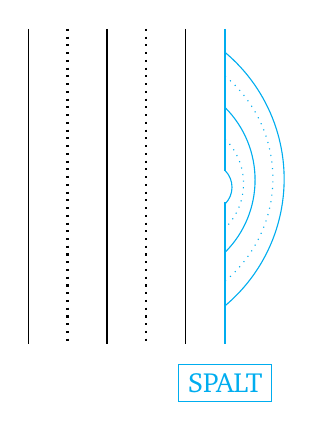
\begin{tikzpicture}
		\draw (2.5,0) -- (2.5,-4);
		\draw[dotted,thick] (3,0) -- (3,-4);
		\draw (3.5,0) -- (3.5,-4);
		\draw[dotted,thick] (4,0) -- (4,-4);
		\draw (4.5,0) -- (4.5,-4);
		\draw[thick,cyan] (5,0) -- (5,-1.8);
		\draw[thick,cyan] (5,-4) -- (5,-2.2);
		\draw[cyan] (5,-1.8) arc (45:-45:0.3);
		\draw[cyan,dotted] (5,-1.4) arc (45:-45:0.8);
		\draw[cyan] (5,-1) arc (45:-45:1.3);
		\draw[cyan,dotted] (5,-0.6) arc (50:-50:1.7);
		\draw[cyan] (5,-0.3) arc (50:-50:2.1);
		\node[draw,cyan] at (5,-4.5) {SPALT};
	\end{tikzpicture}
\end{document}